\documentclass[t]{beamer}

% Load general definitions
% Preamble file - general definitions, package loading, etc.

%=================================
% Load packages
\usepackage{amssymb,amsmath}
\usepackage{graphicx}
\usepackage{url}
\usepackage{tikz}
\usetikzlibrary{mindmap,trees,arrows}
\usepackage{fancyvrb}
\usepackage[portuguese]{babel} 
\usepackage[utf8]{inputenc}
\usepackage{subfigure}
\usepackage{times}
\usepackage[T1]{fontenc}
\usepackage{cancel}
\usepackage{color}
\usepackage{listings}
\usepackage[document]{ragged2e}
\usepackage{hyperref}
\usepackage{listings}


%=================================
% Set mode
\mode<presentation>
{
	\usetheme{Madrid}
	\usecolortheme{structure}
	\useoutertheme{infolines}
	\setbeamercovered{invisible}
}

% Get rid of nav bar
\beamertemplatenavigationsymbolsempty

% Insert frame number at bottom of the page.
\usefoottemplate{\hfil\tiny{\color{black!90}\insertframenumber}} 

%=================================
% Define new commands

\newcommand\Real{{\mathbb{R}}}
%\newcommand{\vi}{\vspace{0.6\baselineskip}}
%\newcommand{\goodgap}{\hspace{\subfigtopskip}\hspace{\subfigbottomskip}}


% Equation environments
\newcommand{\beq}{\begin{equation}}
\newcommand{\eq}{\end{equation}}
\newcommand{\beqs}{\begin{equation*}}
\newcommand{\eqs}{\end{equation*}}
\newcommand{\beqn}{\begin{eqnarray}}
\newcommand{\eqn}{\end{eqnarray}}
% Bold variables
\newcommand{\mbf}[1]{\ensuremath{\mathbf{#1}}}
% Itemization
\newcommand{\bitem}{\begin{itemize}}
\newcommand{\eitem}{\end{itemize}}
\newcommand{\spitem}{\vskip 1em\item}
\newcommand{\bitems}{\begin{itemize}\item}
\newcommand{\benums}{\begin{enumerate}\item}
\newcommand{\eenum}{\end{enumerate}}
% color blocks
\newenvironment{colorblock}[2]{%
\setbeamercolor{block title}{#2}
\begin{block}{#1}}{\end{block}}
% Vertical spacing
\newcommand{\vone}{\vskip 1em}
\newcommand{\vhalf}{\vskip .5em}
% Frame environments
\newenvironment{ftst}[3][t]{%
\begin{frame}{environment=ftst,#1}
\frametitle{#2}
\framesubtitle{#3}}{\end{frame}}
\newenvironment{ftstf}[2]{
\begin{frame}[fragile,environment=ftstf]
\frametitle{#1}
\framesubtitle{#2}}{\end{frame}}
% colors
\definecolor{MyGray}{rgb}{0.5,0.5,0.5}
\definecolor{MyDBGray}{rgb}{0.1,0.1,0.4}
\definecolor{darkgreen}{rgb}{0,0.4,0}
\definecolor{black}{rgb}{0,0,0}
\def\defn#1{{\color{red} #1}}
% Footnote
\renewcommand{\thefootnote}{\alph{footnote}}
% Relaxed footnotes
\newcommand{\lfr}[1]{\let\thefootnote\relax\footnote{\tiny #1}}
% Verbatim environment - using FANCYVRB package
\DefineVerbatimEnvironment%
{rcode}{Verbatim}
{fontsize=\scriptsize}

% Verbatim environment - using LISTINGS package
%\lstnewenvironment{rcode} {\lstset{	language = R,
%									basicstyle = \scriptsize\ttfamily,
%									showspaces = false,
%									showstringspaces = false,
%									showtabs = false,
%									keywordstyle = \color{black}\bfseries,
%									commentstyle = \color{darkgreen},
%									numbers = none,
%									otherkeywords={	<-,
%													ggplot,
%													geom_boxplot,
%													facet_grid,
%													shapiro.test,
%													fligner.test,
%													glht,
%													with},
%									deletekeywords={data,
%													model,
%													residuals,
%													c,
%													axis,
%													default,
%													labels,
%													qq.text}}}%
%{}

% Specific definitions
\title[]{Tópicos Especiais em Computação I}
\subtitle[]{Avaliação de modelos}
\author[]{Patrícia Lucas\\{\footnotesize }}
\institute{Bacharelado em Sistemas de Informação \\ IFNMG  - Campus Salinas}
\date{\scriptsize Salinas\\Março 2021}

\begin{document}

\setbeamertemplate{caption}{\raggedright\insertcaption\par}
% cover page
\setbeamertemplate{footline}{}
\begin{frame}

\begin{center}
\includegraphics[width=.15\textwidth]{}
\end{center}
  \titlepage
  \begin{tikzpicture}[remember picture,overlay]
  \node[anchor=south east,xshift=-5pt,yshift=5pt] at (current page.south east) {\tiny Versão 1.2021};
  \node[anchor=south west,yshift=0pt] at (current page.south west) {
\includegraphics[width=.25\textwidth]{Logos/salinas_horizontal_jpg.jpg}};
  \end{tikzpicture}  
\end{frame}

% Main slides

\begin{ftst}{Referência}{{Avaliação de modelos}}
\begin{figure}
    
\includegraphics[scale=0.35]{Figuras/slide01_11.jpg}
\end{figure}
Capítulo 9: Avaliação de modelos preditivos.
\vone
\scriptsize
Inteligência Artificial: Uma abordagem de aprendizado de máquina. Katti Faceli...[et al.]. - Rio de Janeiro: LTC, 2011.

\end{ftst}

%=====

\begin{ftst}{Visão geral}{Avaliação de modelos}
\justifying
Uma característica particular dos algoritmos de aprendizagem de máquina é a necessidade de experimentação.
\vone
A validação de qualquer técnica de aprendizagem de máquina geralmente envolve a realização de experimentos controlados, em que se demonstre a sua efetividade na solução de diversos problemas, representados por seus conjuntos de dados associados.
\vone
É recomendável seguir procedimentos que garantam a corretude, a validade e a reprodutibilidade dos experimentos realizados e, mais importante, das conclusões obtidas a partir de seus resultados.

\end{ftst}

%=====

\begin{ftst}{Visão geral}{Avaliação de modelos}
\justifying
A avaliação experimental de um algoritmo de aprendizagem de máquina pode ser realizada sobre diversos aspectos: acurácia do modelo, compreensibilidade do conhecimento extraído, tempo de aprendizado, etc.
\vone
Nessa aula, vamos concentrar a discussão em medidas relacionadas ao desempenho obtido nas predições realizadas.
\vone
\begin{itemize}
    \item Métricas de erro para problemas de classificação.
    \item Métricas de erro para problemas de regressão.
    \item Amostragem.
\end{itemize}

\end{ftst}

%=====

\begin{ftst}{Métricas de erro para classificação}{Avaliação de modelos}
\justifying
\textbf{Taxa de erro de classificadores:}
\begin{equation}
    err(\hat{f}) = \frac{1}{n} \sum^n_{i=1} I(y_i \neq \hat{f}(x_i))
\end{equation}

Em que:
\vone
- $I(a) = 1$, se $a$ é verdadeiro e $0$, caso contrário.
\vone
- Dado um conjunto de dados contendo $n$ objetos, sobre o qual a avaliação será realizada, essa taxa equivale à proporção de exemplos desse conjunto classificados incorretamente por $\hat{f}$ e é obtida pela comparação da classe conhecida de $x_i$, $y_i$, com a classe predita, $\hat{f}(x_i)$.
\vone
- A taxa de erro varia entre $0$ e $1$ e valores próximos de $0$ são considerados melhores.


\end{ftst}

%=====

\begin{ftst}{Métricas de erro para classificação}{Avaliação de modelos}
\justifying
\textbf{Acurácia de classificadores:}
\begin{equation}
    ac(\hat{f}) = 1 - err(\hat{f})
\end{equation}
\vone
- Nesse caso, valores próximos de $1$ são considerados melhores.


\end{ftst}

%=====

\begin{ftst}{Métricas de erro para classificação}{Avaliação de modelos}
\justifying
\small
\textbf{Matriz de confusão:} ilustra o número de predições corretas e incorretas em cada classe. Exemplo para um problema com 3 classes:
\begin{figure}
    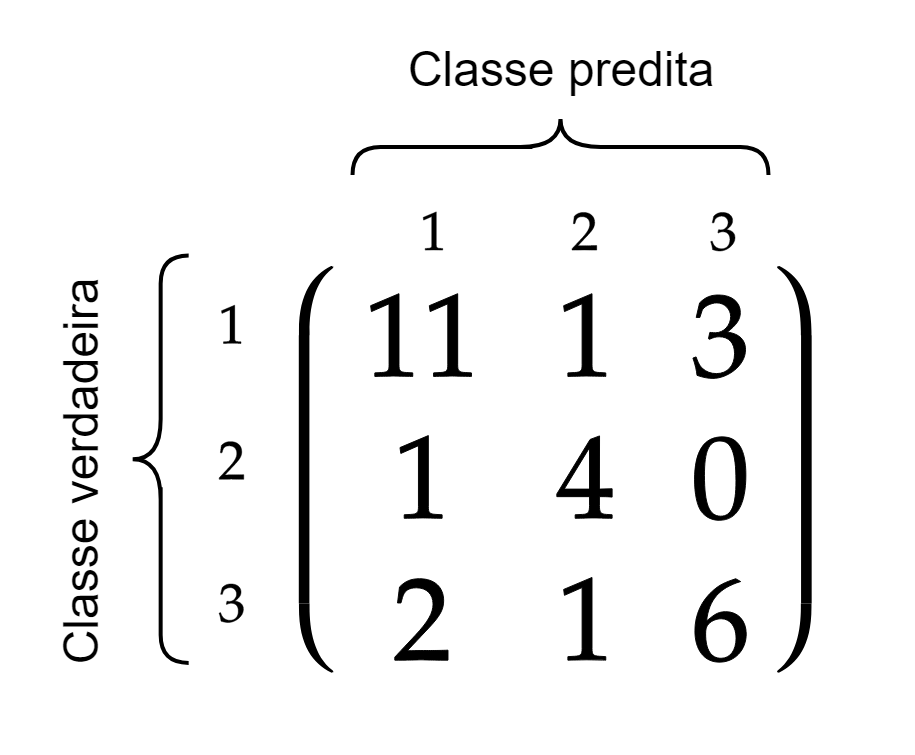
\includegraphics[scale=0.13]{Figuras/slide04_01.png}
\end{figure}
\scriptsize
Temos que:
\vone
- 11 amostras da classe 1 foram classificadas corretamente, 1 incorretamente como classe 2 e 3 incorretamente como classe 3.

- 4 amostras da classe 2 foram classificadas corretamente e 1 incorretamente como classe 1. 

- 6 amostras da classe 3 foram classificadas corretamente, 1 incorretamente como classe 2 e 2 incorretamente como classe 1.

\end{ftst}

%=====

\begin{ftst}{Métricas de erro para classificação}{Avaliação de modelos}
\justifying
\textbf{Matriz de confusão para duas classes:}

\begin{figure}
    \centering
    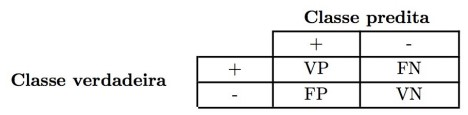
\includegraphics[scale=0.7]{Figuras/slide04_06.jpg}
\end{figure}
\footnotesize
\begin{itemize}
    \item VP: corresponde ao número de exemplos da classe positiva classificados corretamente.
    \item VN: corresponde ao número de exemplos da classe negativa classificados corretamente.
    \item FP: corresponde ao número de exemplos cuja classe verdadeira é negativa mas que foram classificados incorretamente como pertencendo à classe positiva.
    \item FN: corresponde ao número de exemplos originalmente à classe positiva que foram classificados incorretamente como pertencendo à classe negativa.
\end{itemize}

\end{ftst}

%=====

\begin{ftst}{Métricas de erro para classificação}{Avaliação de modelos}
\justifying
\small
\textbf{Análise ROC:} o gráfico ROC é um gráfico bidimensional plotado em um espaço denominado espaço ROC, com eixos X e Y representando as medidas TFP e TVP, respectivamente.

\begin{figure}
    \centering
    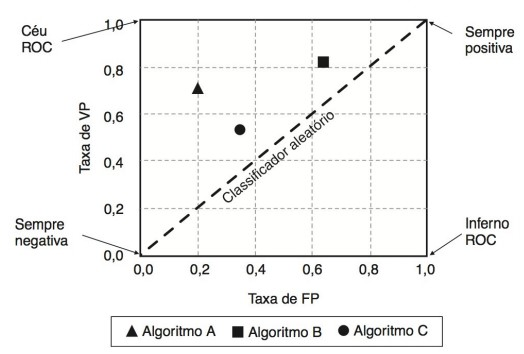
\includegraphics[scale=0.5]{Figuras/slide04_07.jpg}
\end{figure}



\end{ftst}

%=====

\begin{ftst}{Métricas de erro para classificação}{Avaliação de modelos}
\justifying
\small
\textbf{Curva ROC} 

\begin{figure}
    \centering
    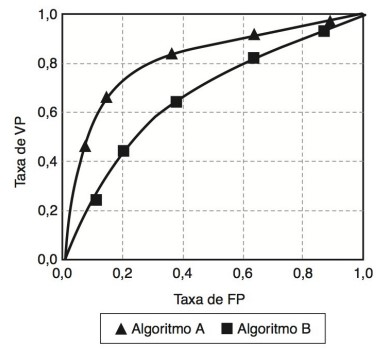
\includegraphics[scale=0.5]{Figuras/slide04_08.jpg}
\end{figure}

\textbf{Área abaixo da curva ROC (AUC):} medida que produz valores entre $0$ e $1$, sendo que os mais próximos de $1$ são considerados melhores.
\end{ftst}

%=====

\begin{ftst}{Métricas de erro para regressão}{Avaliação de modelos}
\justifying
Para problemas de regressão o erro de $\hat{f}$ pode ser calculado pela distância entre o valor $y_i$ conhecido e aquele predito pelo modelo $\hat{f}(x_i)$. 
\vone
As medidas de erro mais utilizadas são o erro quadrático médio (MSE - \textit{mean squared error}) e a distância absoluta média (MAD - \textit{mean absolute distance}):

\begin{equation}
    MSE (\hat{f}) = \frac{1}{n} \sum_{i=1}^{n}(y_i - \hat{f}(x_i))^2
\end{equation}

\begin{equation}
    MAD (\hat{f}) = \frac{1}{n} \sum_{i=1}^{n}|y_i - \hat{f}(x_i)|
\end{equation}

O MSE e MAD são sempre positivos e para ambas as medidas, valores mais baixos correspondem a melhores modelos.

\end{ftst}

%=====

\begin{ftst}{Amostragem}{Avaliação de modelos}
\justifying
\small
Para se obter estimativas de desempenho preditivo mais confiáveis devemos definir um subconjunto de dados de treinamento e um subconjunto de dados de teste.
\vone
O subconjunto de treinamento é usado na etapa de ajuste do modelo, enquanto que o subconjunto de teste é usado para simular a apresentação de objetos novos ao preditor.
\vone
Esses subconjuntos devem ser disjuntos para assegurar que as medidas de desempenho sejam obtidas a partir de um conjunto de exemplos diferente daquele usado no aprendizado.
\vone
No caso de métodos de amostragem que envolvem média de desempenho, deve-se reportar também os valores de desvio padrão associados. Um alto desvio padrão indica uma alta variabilidade nos resultados, ou seja, uma instabilidade.

\end{ftst}

%=====

\begin{ftst}{Amostragem}{Avaliação de modelos}
\justifying
\textbf{Métodos de amostragem \textit{holdout}:}
\vone
\begin{figure}
    \centering
    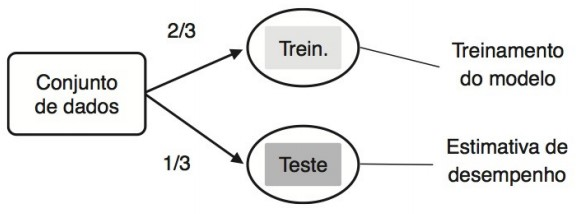
\includegraphics[scale=0.7]{Figuras/slide04_02.jpg}
\end{figure}

Problema: o \textit{holdout} não permite avaliar o quanto o desempenho de uma técnica varia quando diferentes combinações de objetos são apresentados em seu treinamento.

\end{ftst}


%=====

\begin{ftst}{Parâmetros versus Hiperparâmetros}{Escolha do modelo}
\justifying
Um \textbf{parâmetro} de modelo é uma variável de configuração interna ao modelo e cujo valor pode ser estimado a partir dos dados.
\vone
Um \textbf{hiperparâmetro} de modelo é uma configuração externa ao modelo e cujo valor não pode ser estimado a partir dos dados. Hiperparâmetros formam a estrutura do modelo.
\vone
Portanto, caso você esteja trabalhando com uma família única de modelos, como por exemplo MLPs, a escolha do modelo se resume a escolha dos hiperparâmetros que formam a melhor estrutura para um determinado conjunto de dados. 
\vone
Mas como encontrá-los?

\end{ftst}

%=====

\begin{ftst}{Amostragem}{Escolha do modelo}
\justifying
\textbf{Métodos de amostragem por validação cruzada:}
\vone
\begin{figure}
    \centering
    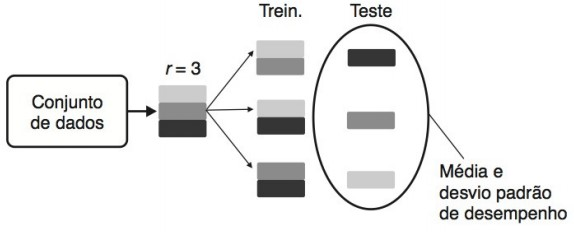
\includegraphics[scale=0.5]{Figuras/slide04_04.jpg}
\end{figure}
\small
O conjunto de dados é dividido em $r$ subconjuntos de tamanho aproximadamente igual. O modelo é treinado usando $r-1$ exemplos e o restante é usado para teste. Esse processo é repetido $r$ vezes, utilizado em cada ciclo uma partição diferente para teste.
\vone
O desempenho final do preditor é a média dos desempenhos observados sobre cada subconjunto de teste.

\end{ftst}

%=====

\begin{ftst}{Amostragem}{Escolha do modelo}
\justifying
\textbf{Validação cruzada com \textit{avaliação fora da amostra}:}

\begin{figure}
    \centering
    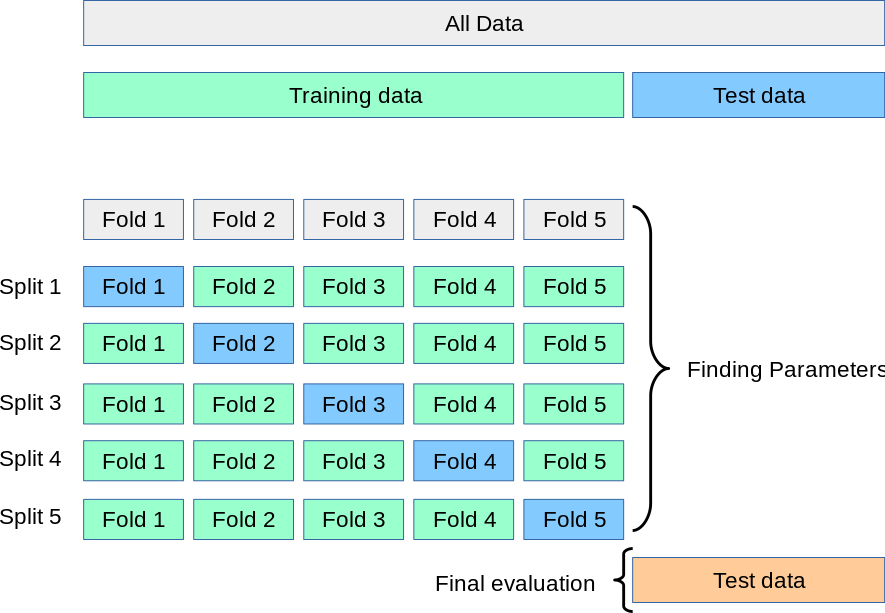
\includegraphics[scale=0.3]{Figuras/cross_validation.png}
\end{figure}



\end{ftst}





\end{document}